% SP1 manuscript draft, 13 Nov 2026. Class: icsthesis.cls (ICS template). Citations: apacite (natbibapa).
% Build: pdflatex main; bibtex main; pdflatex main; pdflatex main
\documentclass{icsthesis}
\usepackage{enumitem}
\usepackage{lipsum} % acknowledgement placeholder only; remove with it
\usepackage{url}
\usepackage{array}
\newcolumntype{L}[1]{>{\raggedright\arraybackslash}p{#1}}
\setlist{nosep}

% Marks results not yet run. Remove every \PENDING before submission.
\newcommand{\PENDING}[1]{\par\noindent\fbox{\parbox{0.95\linewidth}{\singlespacing\small\textbf{PENDING.} #1}}\par}

\renewcommand{\TITLE}{AN AGENT-BASED MODEL OF RED-STRIPED SOFT SCALE INSECT (\emph{Pulvinaria tenuivalvata}) MANAGEMENT ON SUGARCANE IN NEGROS ISLAND}
\renewcommand{\AUTHOR}{JOANNE MARYZ CABATINGAN}
\renewcommand{\DEGREE}{BACHELOR OF SCIENCE IN COMPUTER SCIENCE}
\renewcommand{\MONTH}{NOVEMBER}
\renewcommand{\YEAR}{2026}

\begin{document}

	\begin{frontmatter}
		\maketitle

		% Approval page, per the AY 2026-2027 ICS template (SP version: adviser only).
		\begin{approvalpage}
			\sloppy The Special Problem hereto attached, titled \TITLE , prepared and submitted by \AUTHOR , in partial fulfillment of the requirements for the degree of \DEGREE\ is hereby accepted.

			\addsignature{ZENITH O. ARNEJO}{Adviser}
		\end{approvalpage}

		\begin{biosketch}
			Joanne Maryz Cabatingan is from Dipolog City, Zamboanga del Norte. She finished high school with high honors at the Philippine Science High School -- Zamboanga Peninsula Region Campus in 2023, then moved to Los Ba\~{n}os to take up Computer Science at the University of the Philippines Los Ba\~{n}os as a Department of Science and Technology scholar.

			Away from the screen, she makes charm bracelets, swims, and puts together wooden puzzles. She also likes to travel on her own.

			She hopes to work in user experience design and research, simulation, or software engineering, and later to take a master's degree.

			\addauthorsignaturefield
		\end{biosketch}

		\begin{acknowledgement}
			% Placeholder: J.M. to write after the manuscript is done. Must not exceed one page.
			\lipsum[4]
		\end{acknowledgement}

		\maketableofcontents
		\makelistoftables
		\makelistoffigures

		\begin{abstractwithpageno}
		\setlength{\emergencystretch}{1.5em}
		\\
		\textbf{\AUTHOR}, University of the Philippines Los Ba\~{n}os, \MONTH\ \YEAR. \textbf{\TITLE}
		\\Major Professor: ZENITH O. ARNEJO\\

			% Abstract, revised 18 Nov 2026 from J.M.'s suggested text. Results come from the draft Chapter 4. Must fit one page.
The red-striped soft scale insect (RSSI), \emph{Pulvinaria tenuivalvata}, had affected 72,103 ha of sugarcane on Negros Island by 2 October 2026, 30.1\% of the area planted \citep{SRA2026FOI}. Its effect on yield has not been measured in the Philippines \citep{Guerrero2024}, yet Negros Occidental funds biological control \citep{Bayoran2026} while Negros Oriental planned chemical spraying \citep{Partlow2026}. A systematic review of 30 agent-based pest models found none of a scale insect and none coupling a farmer's choice between biological and chemical control with pest biology.

This study develops an agent-based model of RSSI management in GAMA. Pest development follows Philippine laboratory biology \citep{Guerrero2026} on a 1-ha map of Negros cane \citep{DiTommaso2024}. Over three crop years, under one common treatment trigger, the model compares \emph{no control}, \emph{chemical control} whose efficacy may decline with repeated use, fungal \emph{biological control}, and a \emph{hybrid} that applies the fungus at infestation Levels 1 and 2 and a chemical at Level 3.

Every control strategy cut cumulative pest load at least 82\% below no control. Chemical control matched biological control only if its efficacy halved no faster than about once per 80 applications. The hybrid added nothing while fungal efficacy held, but was best when both agents lost efficacy quickly. The ranking held in 15 of 18 sensitivity cases. A hindcast against SRA data showed baseline spread is too slow. These are comparisons between strategies under stated assumptions, not field predictions.

		\end{abstractwithpageno}
	\end{frontmatter}

	\begin{mainmatter}
		\setlength{\emergencystretch}{3em} % the class disables hyphenation; this stops lines running into the margin
		% Chapter 1. Ported from docs/chapter1-draft.md (15 Oct 2026), updated 13 Nov 2026 for the island landscape.
\section{INTRODUCTION}

\subsection{Background of the Study}

Negros Island is the centre of Philippine sugarcane, with about 57\% of the national sugarcane area \citep{PCAARRDnd}. The crop supports a large and mostly smallholder base, with about 88,000 sugarcane farmers nationally, of whom about 84\% hold less than 5 ha \citep{PCAARRDnd}. An earlier count gives 78,276 farmers and 81.5\% below 5 ha for 2013--2014 \citep{Briones2020}. Shocks to the crop therefore turn quickly into rural income loss.

Since 2022 the industry has faced a new threat, the red-striped soft scale insect (RSSI), \emph{Pulvinaria tenuivalvata} (Newstead) (Hemiptera: Coccidae). RSSI is a sap-sucking soft scale that excretes honeydew, which promotes sooty mould and interferes with photosynthesis \citep{Guerrero2026}. Earlier studies reviewed by \citet{Guerrero2026} report that this feeding reduces cane yield and sucrose content, although no such study has been done in the Philippines \citep{Guerrero2024}. The insect reproduces by thelytokous parthenogenesis, so populations are all female and can build up without mating \citep{Guerrero2026}. Under Philippine laboratory conditions a female lays about 197 eggs, and the cycle from egg to death lasts about 63 days \citep{Guerrero2026}. RSSI was first observed in the Philippines in Bacolor, Pampanga, in June 2022 \citep{Navasero2023}. In Negros it was first noted in northern Negros Occidental in late March 2025 and was declared an infestation on 22 May 2025, when it had spread over 87 ha \citep{ManilaBulletin2025}. By 2 October 2026 the Sugar Regulatory Administration (SRA) had validated 72,103 ha of RSSI-affected sugarcane on Negros Island, about 30\% of the 239,216 ha planted in crop year 2025--2026 \citep{SRA2026FOI}.

Negros Occidental was placed under a state of calamity in July 2025 \citep{Masculino2025} and again on 30 June 2026 \citep{Bayoran2026}, and Negros Oriental followed on 20 July 2026 \citep{Partlow2026}. The response so far has relied on local government units and farmers to deliver control \citep{Partlow2026,Gomez2026}. It includes chemical and drone spraying, biological control with entomopathogenic fungi, and emergency cash assistance \citep{ChiniMandi2026}, quick response funds released under the calamity declarations \citep{Partlow2026}, and the propagation of a variety reported to be more resistant \citep{Gomez2026}. The provincial government of Negros Occidental has declined to fund chemical spraying and has opted for biological control, although it has not banned chemicals \citep{Bayoran2026}. Its Provincial Biosecurity Task Force applies the entomopathogenic fungi \emph{Metarhizium} and \emph{Beauveria}, by truck-mounted mist sprayer where a farm track reaches the field and through farmers' backpack sprayers elsewhere \citep{PGNO2026}, and the province is propagating that variety \citep{Gomez2026}. The task force also surveys infestation in the field. As of 8 November 2026 it had surveyed 16,505 farmlots in all 31 local government units it covers in Negros Occidental: 50\% were rated low, 29\% moderate, and 15\% high, and no RSSI was found in 6\% \citep{PGNO2026}. The survey is a dated snapshot whose coverage has grown over time, so it does not show how infestation has changed. The choice between biological, chemical, and mixed control is being made in real time and at scale, without a published or operationally deployed decision-support tool to compare control strategies before deployment.

\subsection{Statement of the Problem}

The RSSI outbreak in Negros is severe, spreading, and managed reactively, and the central management question, which control strategy to pursue, is being decided without an established quantitative basis. The system is data-poor. The pest's effect on cane yield and sucrose content has not been studied in the Philippines \citep{Guerrero2024}, and the absence of region-specific biological data limits the development of monitoring systems and economic threshold levels \citep{Guerrero2026}. Infestation levels are now defined by insect counts per leaf \citep{PGNO2026}, but no study links those counts to yield loss, so there is still no damage-based threshold for deciding when to act.

Agent-based modelling can represent the pest, the crop, and the farmer as interacting agents and can be used to explore management strategies in silico before they are deployed in the field. A systematic review of the agent-based pest-management literature (Review of Literature) found that, of 30 reviewed models, none models a scale insect or a sugarcane-RSSI system, and none is validated on Philippine field data. No agent-based model for comparing RSSI control strategies on sugarcane has been reported. The problem this study addresses is to build such a model when many of the quantities it needs, such as spread between fields and yield loss, have not been measured, and to compare control strategies while stating clearly which inputs are known and which are assumed.

\subsection{Objectives of the Study}

The general objective is to develop an agent-based model of red-striped soft scale insect management on sugarcane in Negros Island as a tool for exploring pest-management strategies. The specific objectives are as follows.

\begin{enumerate}
	\item To characterise the RSSI-sugarcane-farmer system in Negros from literature and field reports, including pest biology, crop response, control options, and the management context.
	\item To formalise a conceptual model of pest, crop, farmer, and natural-enemy interactions suitable for agent-based implementation.
	\item To identify data sources and to state explicitly what can and cannot be parameterised, treating unsupported quantities as assumptions to be tested.
	\item To implement an initial agent-based model in GAMA.
	\item To evaluate model behaviour through exploratory simulations comparing control strategies (chemical, biological, hybrid, and none) on cumulative pest load, the extent of pest spread over the simulated area, and the number of control applications, with cane yield loss derived from an assumed damage function, allowing the efficacy of chemical control to decline with repeated use so that the strategies are compared over sustained use rather than a single application.
\end{enumerate}

\subsection{Significance of the Study}

The management decision facing the province, biological versus chemical versus hybrid control, is currently made without a way to test strategies before committing resources. A model that represents the system and lets strategies be compared in silico offers a low-cost testbed for that decision. Because chemical efficacy is allowed to fall with repeated use, the comparison also speaks to how each strategy holds up under sustained use, which is the crux of the biological-versus-chemical debate, rather than only to a single season.

The study is also useful for its method. By recording which parameters are supported by data and which are not, it documents what a data-poor, emerging-pest system can and cannot yet support in a model. This record is useful to the SRA and to later researchers.

\subsection{Scope and Limitations}

This study develops a conceptual model and an initial, exploratory agent-based model of RSSI management on sugarcane in Negros. The model is intended for comparing control strategies. Its outputs are relative comparisons between strategies, not calibrated field predictions.

Several quantities cannot be parameterised from available data. Pest life-history parameters come from a single laboratory temperature regime \citep{Guerrero2026}, so the model uses no development function that depends on temperature. No dose-response relates scale density to yield or sugar loss, so the damage function takes an assumed form. Crawler dispersal, stage-specific field mortality, and per-hectare control costs could not be obtained from verifiable sources and are treated as assumptions swept across plausible ranges. Pesticide resistance is not modelled as an evolutionary process. Instead, the efficacy of chemical control declines with cumulative use at an assumed rate, so that the long-run disadvantage of repeated spraying is represented without genotype-level data, which were not found for RSSI. Because these quantities are uncalibrated, the model is assessed with a hindcast against one verified Negros figure, not by statistical fitting.

The study is limited to RSSI on sugarcane in Negros and to the comparison of chemical, biological, hybrid, and no-control strategies. The landscape covers all of Negros Island at 1-ha resolution and is built from a satellite sugarcane map for 2019--2022 \citep{DiTommaso2024}. That map predates the outbreak and overstates the area planted in 2025--2026, the SRA reply included no infestation map, because mapping is still ongoing, and no key linking municipal records to mill districts \citep{SRA2026FOI}, and the provincial survey records are viewable but not released as data \citep{PGNO2026}. The model therefore starts from 87 infested cells placed at random within the municipalities first reported as affected and is not used to say where the pest will spread next. Re-invasion from outside the island is outside the scope of the study. Reported losses of up to 50\% of cane yield and sugar content \citep{ChiniMandi2026} are treated as claims from news sources, not as established measurements, because no primary study is cited for them.

\subsection{Dataset}

The study does not use a single measured dataset. It assembles parameters and context from published literature, government and industry sources, open geospatial data, and news reports. Each item is recorded with its source and a status of real, analogue, or assumption in the study's parameter table.

Pest biology, the best-supported component, comes from \citet{Guerrero2026}, which gives stage durations, fecundity, reproduction mode, and longevity for a Philippine laboratory population. Control efficacy has Philippine anchors. \emph{Metarhizium anisopliae} caused 86.67\% to 91.11\% mortality at 15 days in vitro \citep{Buletin2026}. Natural parasitism of teneral and young adults was 34.85\% in a screenhouse and 66.8\% in the field in Luzon \citep{Guerrero2024}. The cropping calendar comes from \citet{MojicaSevilla2025}: the crop year runs from October to September, and planting runs from October to May. Negros cane yield and planted area by mill district for crop years 2020--2021 to 2025--2026, sugar recovery for 2025--2026, and the validated RSSI-affected area by municipality as of 2 October 2026, come from the SRA reply to a freedom-of-\allowbreak information request \citep{SRA2026FOI}. Across the 12 Negros mill districts, cane yield ranged from 49.32 to 71.64 tonnes per hectare over crop years 2020--2021 to 2024--2025, and Negros as a whole recorded 59.48 tonnes per hectare and a sugar recovery of 1.61 LKg per tonne of cane in 2025--2026 \citep{SRA2026FOI}. The definitions of infestation Levels 1 to 3 and the current severity of infestation in Negros Occidental come from the provincial monitoring dashboard \citep{PGNO2026}, an official operational source that is dated and subject to revision. The landscape uses the 10-m sugarcane map of \citet{DiTommaso2024}, municipal boundaries from the OCHA common operational dataset \citep{OCHA2025}, and roads from OpenStreetMap \citep{OSM2026}. Sugar prices and the farm-size distribution give context but are not model inputs, because farm income is not modelled.

The dataset has notable gaps. No economic injury level, economic threshold, or damage function was found for RSSI, and the lack of region-specific biological data limits their development \citep{Guerrero2026}. The provincial dashboard describes damage that worsens with severity, with yield able to fall at high severity, but it gives no measured relation \citep{PGNO2026}. Per-hectare control costs, the farmgate cane price, and labour costs were not found in verifiable sources. The SRA reports that its mapping is still ongoing \citep{SRA2026FOI}, and the provincial survey is a single dated snapshot, so no multi-date infestation series was found. Climate is held out of the model, so development runs at the laboratory rate of \citet{Guerrero2026}. No resistance or efficacy-loss data were found for RSSI, so the decline in chemical efficacy with repeated use is set as an assumption. These gaps define the parameters that are handled as assumptions and tested by sensitivity analysis rather than presented as data.

		\section{REVIEW OF LITERATURE}

\subsection{Overview}

This section reviews the related literature through a systematic review, which identifies, screens, and selects studies by a documented and repeatable procedure rather than by narrative selection. A narrative review reports what a few chosen studies do, but it cannot show what the field as a whole has left undone, and a new model must be justified against that undone work. A systematic procedure makes both the body of studies retained for analysis, hereafter the corpus, and the research gap it reveals defensible.

The review concerns agent-based models (ABMs), simulations in which individual entities such as pests, crops, and farmers are represented as interacting agents, applied to insect pest management. It addresses three questions. First, what agent-based models exist for insect pest management, and how are they built? Second, along the dimensions that matter for a soft-scale model on sugarcane, how is the field distributed, and which modelling options are common, rare, or absent? Third, where in that distribution does a model of RSSI fall, and what does it contribute that no reviewed model provides?

\subsection{Review Method}

The review followed the PRISMA 2020 guidelines \citep{Page2021} for identification, screening, and selection, so the path from raw records to the final studies is logged and reproducible. The analytical organisation, described in the next subsection, codes each study against published typologies of model structure, agent architecture, and validation \citep{Taillandier2019,Wooldridge1995,Rykiel1996}.

The search covered two databases, Web of Science and Scopus. The query combined three concept blocks: a modelling-method block (agent-based, individual-based, multi-agent), a pest-and-management block, and an agricultural-context block. The same finalised string was run in both databases, differing only in field-tag syntax (Web of Science TS=, Scopus TITLE-ABS-KEY), with no date or document-type filters.

The two databases returned 426 records, 125 from Web of Science and 301 from Scopus. Removing 117 duplicates left 309 unique records. Title-and-abstract screening excluded 262 records and selected 47. The inclusion criterion required a record to describe an agent-based or individual-based model of an insect pest and its management in an agricultural or comparable setting. Full-text review of the 47 excluded 17 further studies and retained 30. Table~\ref{table:exclusions} categorises every exclusion against that single criterion. The 262 abstract-screening exclusions fall into four types: records off-topic on an incidental keyword match, such as materials-chemistry, life-cycle-assessment, and remote-sensing papers (about 39\%), studies of a system that is not an insect crop-pest, such as birds, livestock, weeds, or disease vectors (about 36\%), relevant insect-pest agent models too thin to warrant full-text review (about 19\%), and pest studies using a non-agent method, such as a statistical risk index or a differential-equation population model (about 5\%). The largest full-text exclusions are reviews rather than primary models and studies whose model focus is out of scope, such as resistance genetics or beneficial-insect dynamics. A third group is redundant restatements of one wind-borne aphid dispersal model, of which two were kept to represent it \citep{Wang2019,Koralewski2022} and four close repeats were dropped. The remaining exclusions are software or educational models and one non-agent reaction-diffusion model. Each final study carries its source database, duplicate status, screening decision and reason, full-text decision, and analytical codes, so the funnel from 426 to 30 can be audited.

\begin{table}[!htbp]
\vspace{2ex}
\centering
\caption{Exclusion categories against the single inclusion criterion (an agent-based or individual-based model of an insect crop-pest and its management).}
\label{table:exclusions}
\begin{tabular}{llr}
\hline\hline
Stage & Exclusion type & Count \\ \hline
Abstract (262) & Off-topic incidental keyword match & about 39\% \\
 & Not an insect crop-pest system & about 36\% \\
 & Relevant pest ABM, too thin for full text & about 19\% \\
 & Not an agent-based method & about 5\% \\
Full text (17) & Review or synthesis, not a primary model & 5 \\
 & Out-of-scope focus & 5 \\
 & Redundant restatement of a retained aphid model & 4 \\
 & Software package or educational model & 2 \\
 & Not an agent-based or individual-based model & 1 \\ \hline\hline
\end{tabular}
\vspace{2ex}
\end{table}

\begin{figure}[!htbp]
\begin{center}
	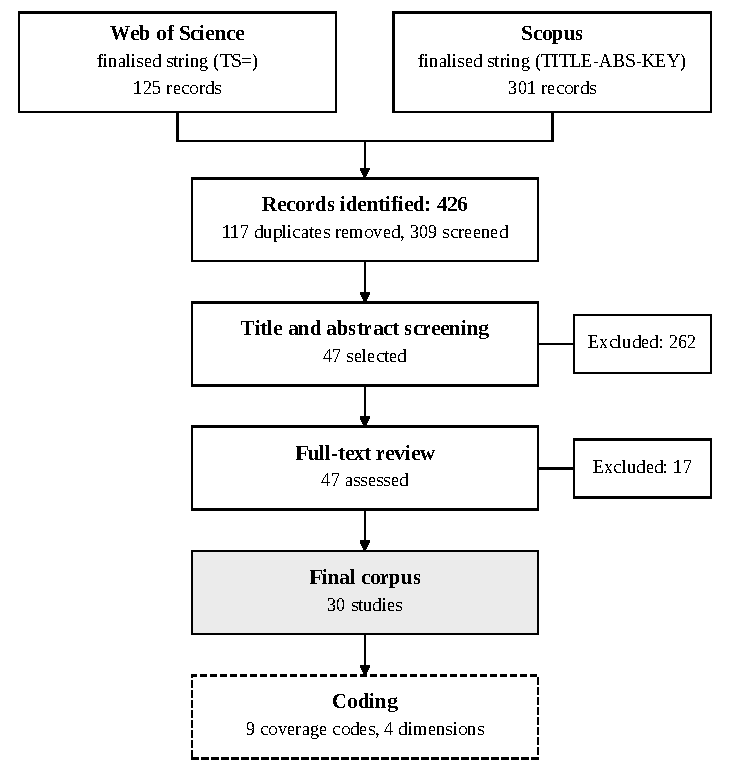
\includegraphics[width=0.9\textwidth]{figures/fig-slr-flow}
	\caption{Flow of the systematic review, from 426 database records through duplicate removal, abstract screening, and full-text review to the 30 final articles.}
	\label{fig:slrflow}
\end{center}
\end{figure}

\subsection{Analytical Framework}

Each of the 30 final studies was coded in two ways. The first is a set of nine coverage codes recording, for each study, the presence or absence of a feature relevant to an RSSI model: a reusable ABM structure, control-strategy testing, model validation, damage-to-yield coupling, temperature or weather drivers, spatial spread, biological control, chemical control, and a farmer decision agent. These codes record whether the field has addressed each component the proposed model needs.

The second is a set of four analytical dimensions. Each dimension takes a published typology together with its full set of values, so a value that no study occupies appears as an empty cell. Spatial representation uses the environment topologies available in the GAMA platform as catalogued by \citet{Taillandier2019}: grid, graph, and continuous. The grid is split by georeferencing. An abstract grid, a schematic lattice of placeless cells, is distinguished from a raster, the same cells tied to a real landscape through a GIS layer, because an RSSI model of actual Negros fields needs the georeferenced kind. A non-spatial value covers models with no explicit environment. Agent architecture uses the reactive, deliberative, and hybrid distinction of \citet{Wooldridge1995}. Validation type uses the distinction between output validation, in which simulated outputs are matched to observed data, and structural validation, in which the model's mechanisms are checked, for example by experts or stakeholders \citep{Rykiel1996}. The farmer decision dimension uses a scheme defined from the corpus, separating behavioural, economic-optimisation, and empirical-rule models from studies with no farmer agent. Coding the corpus against fixed, externally defined value sets records where the field is dense and where it is empty.

Host crop, pest taxonomic group, and modelling platform are recorded as descriptors. The crop labels a study but does not distinguish a modelling choice, so it is reported in the corpus characterisation that follows.

\subsection{The Corpus}

The 30 studies confirm that agent-based pest modelling is an established genre. All 30 carry a reusable ABM structure, which follows from the inclusion criterion. Spatial spread is represented in 21 studies, model validation in 20, and control-strategy testing in 18, so the field is well developed on where a pest is, how it moves, and whether the model was checked. Temperature or weather drivers appear in 15 studies and a damage-to-yield coupling in 12. The two control levers this study contrasts are each present in about a third of the corpus, biological control in 11 studies and chemical control in 9. The least common feature is a farmer modelled as a decision agent, in 8 of the 30.

Sugarcane is a minority setting. Of the 30 studies, five model sugarcane \citep{Alves2024,Alves2026,vanVuuren2018,Human2023,Potgieter2025}, and all five model stalk borers or a weevil. Tree or fruit crops account for 5 studies, field or row crops for 14, and 2 are set outside a cropping system. The remaining 4 are generic. The pest taxonomy is the decisive descriptor. Lepidopteran borers and miners account for 10 studies, Coleoptera for 3, mobile hemipteran sap-suckers such as whitefly, aphid, and lanternfly for 6, Diptera for 2, Orthoptera for 1, and plant disease for 2, with 6 focused generically on natural enemies or farmer behaviour. No study models a scale insect of the superfamily Coccoidea, the group that contains RSSI. The nearest modelled hemipterans are mobile, and RSSI is sessile.

Platforms concentrate on NetLogo, named in 13 of the 30 studies. A further 13 studies used other named environments, including AnyLogic \citep{vanVuuren2018}, Python \citep{Human2023,Potgieter2025}, Delphi \citep{Gergs2026}, MPMAS \citep{Grovermann2017}, and CORMAS \citep{Rebaudo2011,RebaudoDangles2011}. The remaining 4 named no platform. No reviewed study uses GAMA.

The closest precedents to the proposed model cover the two halves of what an RSSI management model needs. \citet{Alves2026} modelled the sugarcane weevil \emph{Sphenophorus levis} in NetLogo. Their model coupled pest density to crop damage through a function that converted biomass loss to a percentage field loss and then to a monetary loss per hectare, switched development between two climate periods defined by local temperature and precipitation, and compared biological-control schemes against an uncontrolled baseline. It supplies the damage-function and economic side on the correct host crop, for a borer and with no farmer agent. For the spatial and validation side, \citet{Koralewski2022} and \citet{Wang2019} modelled the sugarcane aphid as an area-wide, weather-driven dispersal process on a gridded landscape and evaluated the forecasts against infestation observations. None of these models a scale insect, none uses GAMA, and none gives the farmer a decision. Between them they show that the damage-coupling, weather, spread, and validation components the proposed model needs have precedent in the corpus.

Two further models, outside the corpus, illustrate techniques relevant here. \citet{Anderson2015} modelled the spread of the emerald ash borer in a GIS-integrated Repast environment, calibrated against an observed rate of spread and validated against infestation records with 72\% spatial agreement, a clear example of output validation on spatial data. \citet{Wang2015} represented insect distribution within the plant at the leaf and canopy scale, an analogue to RSSI's leaf-position preference. Neither met the agricultural-context search criteria that define the corpus. The first is a forest pest and the second is a conference paper on within-plant behaviour.

\subsection{Synthesis}

Reading the corpus through the four dimensions shows a field concentrated in a few conventional choices and thin or empty elsewhere.

Spatially, 23 of the 30 studies use a grid, 17 abstract patch grids and 6 georeferenced rasters, which is the native representation in GAMA. Grids were used at scales from a single 1-ha field divided into cells \citep{Alves2024} to a region of about 1,750,000 km$^2$ divided into cells of 0.5$^{\circ}$ latitude by 0.5$^{\circ}$ longitude carrying crop and weather attributes \citep{Wang2019}. Continuous space appears in two studies, the locust hopper-band model of \citet{Bernoff2020} and the \emph{Eldana} model of \citet{vanVuuren2018}. A graph or network appears in one study, the multi-pathway spread model of \citet{McNitt2019}. The remaining four studies are non-spatial \citep{Grovermann2017,Gergs2026,Herbillon2024,Chen2024}. Every topology in the typology has at least one example. The single network model used a coarse trade-pathway graph linking regions and did not represent the field-to-field connectivity that cane cutting and haulage involve, so that application remains open.

In agent architecture, 22 of the 30 models are reactive. Pests and natural enemies respond to the current state of their environment without internal plans. Deliberative and hybrid architectures appear only in the 8 studies that model a farmer: one deliberative optimisation model \citep{Grovermann2017} and seven hybrid behavioural models, among them the Rebaudo and Pacilly studies, \citet{Bourceret2024}, and \citet{Chen2024}. The more developed decision machinery in the field is confined to the farmer side and has not been joined to a detailed pest-biology model.

Validation concentrates on the output type. Output validation was done in 16 studies, for example evaluating area-wide dispersal forecasts against infestation observations \citep{Koralewski2022}, validating a whitefly model against field-trial data from several locations in India \citep{Gergs2026}, and checking a fall-armyworm model against county field data \citep{Garcia2019}. Structural or participatory validation appears in 4 studies, including the expert-entomologist review of \citet{Potgieter2025} and the farmer workshops of \citet{Pacilly2019b}. A further 10 studies reported no validation beyond internal sensitivity analysis. Output validation on field data is the mainstream route, and a participatory or face-validation check is uncommon.

The farmer decision dimension is the sparsest. Of the 30 studies, 8 model a farmer decision agent: 6 behavioural, 1 economic-optimisation, and 1 empirical-rule. The behavioural models grounded the decision in a social or diffusion theory, as in the information-diffusion and cooperation models of \citet{Rebaudo2011}, \citet{RebaudoDangles2011}, and \citet{Rebaudo2013}, and the social-ecological model of \citet{Pacilly2019a}. The economic-optimisation model maximised a farm objective function under constraints \citep{Grovermann2017}. The empirical-rule model derived decisions from observed grower behaviour \citep{Chen2024}. The other 22 studies have no farmer agent and treat control as an externally set scenario.

Both control levers are modelled, usually one at a time. Biological control was represented as a natural-enemy or parasitoid mechanism \citep{vanRoermund1997,Collard2018,Delattre2019} or as a sterile-insect or microbial scheme \citep{Diouf2022,Herbillon2024}. Chemical control appeared as spraying regimes or pesticide-use accounting \citep{Grovermann2017}. An explicit comparison of a biological option against a chemical option, scored as a single decision, is uncommon in the corpus.

\subsection{The Research Gap}

The review locates three gaps, stated in decreasing order of how firmly the corpus establishes each one.

The first is the absence of a scale-insect model. No study among the 30 models a scale insect, whose crawlers settle on the host to feed \citep{Guerrero2026}, and the five sugarcane studies all model a borer or a weevil. There is no agent-based model of RSSI, or of any soft scale, on sugarcane, and none validated on Philippine or Negros field data. The nearest modelled hemipterans, cotton whitefly, sugarcane aphid, and spotted lanternfly, are mobile. Sessility is the decisive difference for a model. In an agent-based pest model, movement and spatial spread are core agent behaviours, and a scale insect disperses only briefly as a first-instar crawler before settling permanently on the plant, so dispersal rules written for a mobile whitefly or aphid do not carry over. A model of RSSI must be built new rather than reparameterised from an existing one.

The second is a structural gap at the intersection of the coding dimensions. Of the 30 studies, 8 model a farmer decision and 11 model biological control. No single study couples a farmer decision with both a biological-control option and a pest-biology component. The nearest study, \citet{Chen2024}, gave farmers a choice between biological and chemical control and carried no pest-biology component. The studies that couple a farmer decision to a pest-biology component, such as \citet{Grovermann2017}, modelled only chemical control. This claim rests on the per-study codes rather than on a single tabulated value.

The third concerns methods the field underuses. The single network model represents a coarse regional trade graph and leaves the field-to-field connectivity relevant to cane transport unaddressed. Although grids dominate the corpus, only 6 of the 30 studies use a georeferenced grid whose cells map to a real landscape. Structural or participatory validation is rare, in 4 of the 30 studies.

\subsection{Positioning of This Study}

The proposed model contributes on four points, each located in an empty or thin region of the review. It models RSSI, a scale insect absent from the corpus, on sugarcane, a crop present in 5 of the 30 studies. It gives the farmer a choice between biological and chemical control on top of a pest-biology model, a combination no reviewed study provides. It is implemented in GAMA, a platform no reviewed study uses, on a georeferenced grid of the actual Negros cane landscape, a representation used by only 6 of the 30 studies. Because no Negros infestation time series was found \citep{SRA2026FOI,PGNO2026}, its validation is limited to a hindcast against one verified observation (see Methodology), and output validation on field data is deferred until such data become available.

		\section{METHODOLOGY}

\subsection{Overview of the Approach}

This study builds an agent-based model of RSSI management on sugarcane and uses it to compare four control strategies under sustained use: no control, chemical control, biological control, and a hybrid of the two. The model is exploratory. It is meant to show how the strategies rank under stated assumptions and how sensitive that ranking is to the assumptions that no source supports. It is not meant to predict infestation in any particular Negros field.

The work proceeds in three stages. Pre-modelling consists of the systematic review in the Review of Literature, the collection of data from the SRA and interviews, and the extraction of parameters with an explicit record of what the data cannot support. Model development consists of the conceptual model, its formal description, and its implementation in the GAMA platform \citep{Taillandier2019}. Verification and scenario exploration consist of code checks, the strategy experiments, and a hindcast against the SRA record of the outbreak. GAMA was chosen because grid and raster environments are the commonest representation in the reviewed models, GAMA handles them natively together with GIS layers, and no reviewed study used it.

\subsection{Conceptual Model}

The conceptual model was set out with the PARDI method (Problem, Actors, Resources, Dynamics, Interactions), which builds on the ARDI method of \citet{Etienne2011}. The problem is to determine which control strategy best manages RSSI on sugarcane over sustained use. The boundaries are kept narrow: RSSI on sugarcane only, the cane landscape of Negros Island, daily time steps over three crop years after the first infestation, and a relative comparison between strategies as the output. Resistance evolution at the genotype level and re-invasion from outside the island are out of scope. Resistance to chemicals enters only as a decline in chemical efficacy with repeated use, stated as an assumption.

Three actors matter in the system. Farmers observe infestation and choose a control action. Government bodies (the SRA, the Department of Agriculture, and local government units) fund and deliver control \citep{ChiniMandi2026,Partlow2026}, which the model represents through the hybrid strategy rather than as an agent. Mills and the sugar market set the prices that turn cane into income. The model leaves money out. No source gives a verifiable control cost per hectare, and revenue would be a constant multiple of cane, so the model reports applications by type in place of cost.

\begin{figure}[!htbp]
\begin{center}
	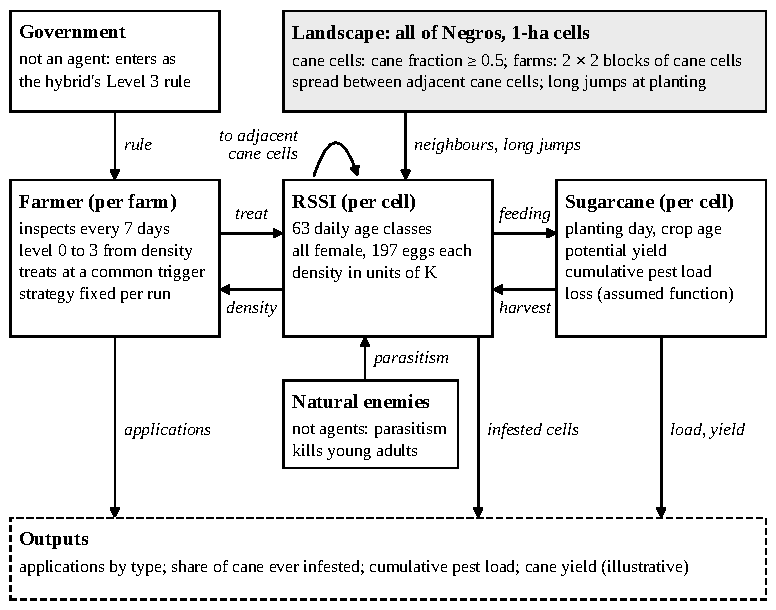
\includegraphics[width=\textwidth]{figures/fig-conceptual}
	\caption{Conceptual model. Pest, crop, and farmer are represented explicitly. Natural enemies and government enter as rules, not agents. Spread runs from an infested cell to its adjacent cane cells (loop). Arrows to the outputs show where each output is computed. Long jumps occur at planting and at ratooning. Harvest removes 90\% of the pest in a cell, an assumed value. Climate is held out.}
	\label{fig:conceptual}
\end{center}
\end{figure}

\subsection{Model Description}

The model is described with the ODD+D protocol \citep{Muller2013}. This section gives the structure. The full description, including every submodel, is kept in the project repository (\texttt{docs/model-odd-d.md}).

\subsubsection{Entities, landscape, and scales}

The landscape covers all of Negros Island, both provinces, at 1-ha resolution (Table~\ref{table:landscape}, Figure~\ref{fig:landscape}). It is a grid of 1,327 by 2,224 cells of 100 m by 100 m in UTM zone 51N, of which 1,278,239 cells lie inside the boundaries of the island's 57 cities and municipalities \citep{OCHA2025}. Each cell carries its municipality and its cane fraction, the share of its 10-m pixels mapped as sugarcane in the global sugarcane map of \citet{DiTommaso2024}, which classifies sugarcane from GEDI lidar and Sentinel-2 imagery over 2019--2022. A cell is a cane cell if its cane fraction is at least 0.5, so that every cane cell is mostly cane. This rule gives 356,869 cane cells. The count is sensitive to the rule (see Limitations of the Method). A 1-ha cell aggregates 100 pixels of the 10-m map. Farm size is not resolved: about 84\% of Philippine sugarcane farmers hold less than 5 ha \citep{PCAARRDnd}, but the share below 1 ha is not reported. Only cane cells hold a crop and a pest. All other cells are inert, and neighbour spread runs only between adjacent cane cells. The grid has a Moore neighbourhood.

The mapped cane area is larger than the area SRA reports as planted. The map gives 351,987 ha of cane on Negros against 239,216 ha planted in crop year 2025--2026, a ratio of 1.47 \citep{SRA2026FOI}. The ratio is 1.36 in Negros Occidental and 1.99 in Negros Oriental. Shares in this study are therefore shares of mapped cane cells, not of planted area, and the hindcast compares hectares by counting one cane cell as 1 ha (see Hindcast).

Roads come from OpenStreetMap \citep{OSM2026}. Trunk, primary, and secondary roads were retained, and cane cells within 100 m of one are flagged as roadside. The roadside flag can raise the long-jump probability of a cell (see Spread). At baseline its multiplier is 1 and the daily roadside inoculation is 0, so roads have no effect on the runs reported here.

\begin{figure}[!htbp]
\begin{center}
	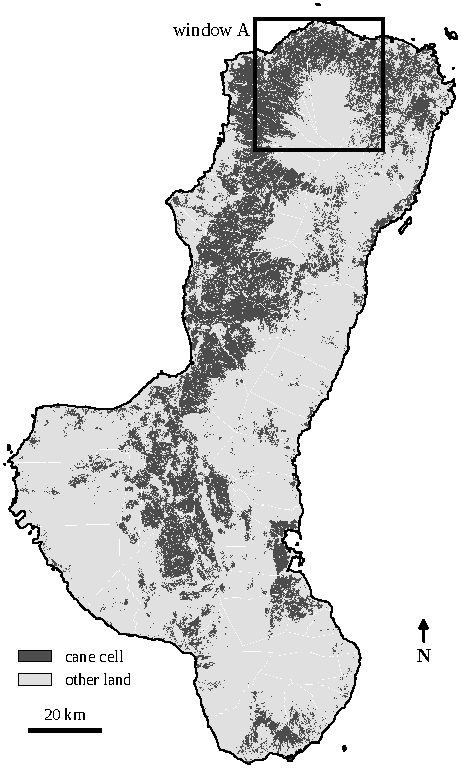
\includegraphics[width=0.55\textwidth]{figures/fig-landscape}
	\caption{Model landscape. Cane cells are 1-ha cells in which at least half the area is mapped as sugarcane in the 2019--2022 map of \citet{DiTommaso2024}. White lines are municipal boundaries \citep{OCHA2025}. The box marks window A (Cadiz City, Manapla, and the City of Victorias), used for the sensitivity analysis.}
	\label{fig:landscape}
\end{center}
\end{figure}

\begin{table}[!htbp]
\vspace{2ex}
\centering
\caption{Landscape inputs and their derived sizes. Counts are computed from the model input grids.}
\label{table:landscape}
\begin{tabular}{L{0.32\textwidth}L{0.6\textwidth}}
\hline\hline
Item & Value and source \\ \hline
Sugarcane & 10-m map, 2019--2022, CC BY 4.0 \citep{DiTommaso2024,DiTommaso2024data} \\
Municipal boundaries & COD-AB version 03, valid 13 February 2025 \citep{OCHA2025} \\
Roads & OpenStreetMap trunk, primary, secondary, downloaded 8 November 2026, ODbL \citep{OSM2026} \\
Grid & 1,327 $\times$ 2,224 cells of 1 ha, UTM zone 51N \\
Cells inside the 57 LGUs & 1,278,239 \\
Cane cells (cane fraction $\geq$ 0.5) & 356,869 \\
Farms (2 $\times$ 2 blocks of cane cells) & 112,713, of 1 to 4 ha \\
Sensitivity window A & Cadiz City, Manapla, City of Victorias: 32,335 cane cells, 10,611 farms \\ \hline\hline
\end{tabular}
\vspace{2ex}
\end{table}

One tick is one day. Day 0 is 1 October, the start of the planting window. The landscape runs free of the pest until the infestation is seeded on day 233, and a run then lasts 1,095 days, three crop years, to day 1,328 (see Initial conditions). A day is the finest scale at which any modelled process changes. The shortest developmental stages last 2 to 6 days, treatments are datable to a day, and egg incubation, the shortest life-history stage, would be skipped by a weekly step.

Each cane cell holds a crop and a pest population. The crop has a planting day, an age, a potential yield, a cumulative pest load, and a loss fraction. The pest is stage-structured and held as a density in each daily age class from 0 to 62 days, in units of the cell's carrying capacity $K$. A cohort representation was chosen over individual insects because each female lays about 197 eggs, and several generations of individuals would be too many agents to run. Farmers are agents. No farm-boundary data were found, so a farm is the set of cane cells in each 2 by 2 block of the grid, which gives 112,713 farms of 1 to 4 ha [assumption]. Each farmer has a level of infestation, a count of applications, and a current chemical efficacy. Natural enemies are not entities. Parasitism enters as a daily mortality term on young adults.

\subsubsection{Process schedule}

Each day the model executes nine steps in a fixed order, each over all cells before the next (Figure~\ref{fig:schedule}). The steps are calendar and crop (planting on a day drawn uniformly from the October to May window, harvest at crop age 365 days, then ratoon regrowth), pest ageing, reproduction, mortality from parasitism and from active treatments, spread, damage, farmer monitoring every 7 days, control, and recording of outputs. Control follows monitoring, so a farmer acts on the day an infestation is detected. To keep island-scale runs tractable, the code visits only the cells where something happens on a given day. This event-driven bookkeeping gave the same results as a full daily scan on window A with a fixed seed.

\begin{figure}[!htbp]
\begin{center}
	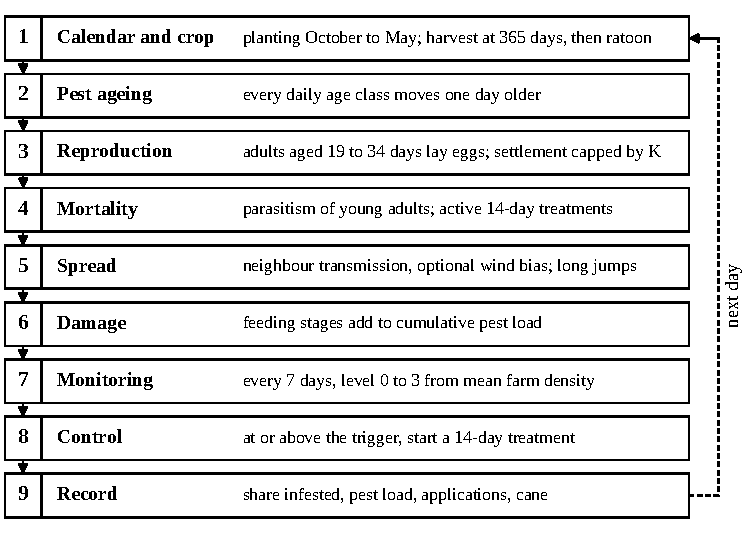
\includegraphics[width=0.85\textwidth]{figures/fig-schedule}
	\caption{Daily process schedule (one tick equals one day). Farmers monitor every 7 days, and each treatment acts for 14 days.}
	\label{fig:schedule}
\end{center}
\end{figure}

\subsubsection{Pest submodel}

Development is deterministic. Stage durations are fixed at the Philippine laboratory values at 27 to 29\,$^{\circ}$C \citep{Guerrero2026}, as one integer set chosen inside every reported range and summing to the reported 63-day cycle from egg to death: egg 2 days, three instars of 6, 6, and 5 days, then young, mature, and senescing adult stages of 13, 17, and 14 days (Figure~\ref{fig:lifecycle}). Reproduction is all-female. Females lay at adult ages 19 to 34 days, 197 eggs in total, taken as 12.31 eggs per day over 16 days. Settled recruits equal eggs multiplied by a settlement survival and by a density-dependent term, one minus the density of feeding stages over $K$. Settlement survival lumps egg, crawler, and settlement losses into one free parameter because no stage-specific field mortality has been measured. Climate is held out. Development runs at the single laboratory rate of \citet{Guerrero2026}.

\begin{figure}[!htbp]
\begin{center}
	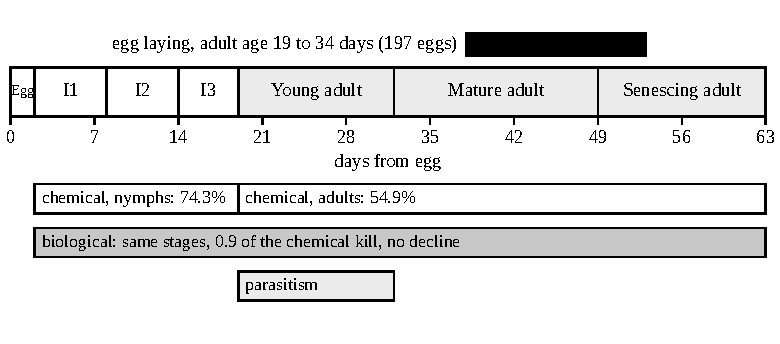
\includegraphics[width=\textwidth]{figures/fig-lifecycle}
	\caption{RSSI life cycle as coded, from egg to death in 63 days \citep{Guerrero2026}, and the stages each control acts on. Chemical kill fractions are medians of six compounds on first application \citep{SRAnd}, applied in the model over 14 days. Shaded stages are adults.}
	\label{fig:lifecycle}
\end{center}
\end{figure}

\subsubsection{Spread}

RSSI adults are fixed to the leaf and crawlers move only within the plant, so the model gives the insect no dispersal distance. An RSSI researcher interviewed for this study stated that between-field spread is driven by external factors and that no rate can be calculated (G.~A.~S. Burgonio, personal communication, 21 September 2026). The model therefore uses two mechanisms with swept, unsourced parameters. In neighbour transmission, a planted cane cell receives crawlers with probability $1-\exp(-\beta P)$, where $P$ is the summed density of its infested cane neighbours on the previous day and $\beta$ is a transmission rate. A wind bias can weight each neighbour by $\max(0, 1 + b\cos(\theta-\phi))$, where $\theta$ is the direction from the neighbour to the cell and $\phi$ is the direction the wind blows toward. The direction is set to the annual prevailing wind at Dumaguete, from the north-east \citep{PAGASAnd}, the only official 1991--2020 normals found for the island. The strength $b$ is 0 at baseline and is tested at 0.5 and 1. Long jumps stand for planting material and cane transport. At planting and at ratooning, a cell may be inoculated with a probability proportional to the share of cane cells currently infested, multiplied for roadside cells by the roadside factor. Both mechanisms are assumptions. They are the least parameterised part of the model, and the sensitivity analysis treats them accordingly.

\subsubsection{Damage}

Damage follows the structure of the closest sugarcane precedent \citep{Alves2026}, in which each pest removes a unit of the crop attribute per step. Each day the feeding stages (ages 2 to 62 days) add to the cell's cumulative pest load, in capacity-days (K-days). Loss is linear in the load accumulated by the current crop and capped at a maximum, with a saturating form available as a robustness check. The slope is set by an interpretable anchor: a cell held at capacity for a whole crop year loses 30\% of yield. No Philippine study has quantified RSSI yield loss \citep{Guerrero2024}, so this coupling is assumed. The provincial dashboard describes visible damage from moderate severity and possible yield loss at high severity \citep{PGNO2026}. This is consistent with loss that rises with pest density, but it gives no values. Two consequences follow and are stated here so that they are not mistaken for findings. Under linear damage, the strategy ranking by yield loss equals the ranking by cumulative pest load whatever the slope, so cumulative pest load and the share of cane ever infested are the primary outputs and cane yield is an illustrative rescaling. Sugar is cane multiplied by a constant recovery, so sugar cannot respond to the strategy and is not reported.

\subsubsection{Control and the farmer decision}

Farmers follow a fixed reactive rule. Every 7 days a farmer reads the mean pest density over its planted cells and assigns an infestation level from 0 to 3. The levels follow the provincial task force, which defines Levels 1 to 3 as 1 to 5, 6 to 10, and more than 10 insects per leaf \citep{PGNO2026}. The model holds density in units of the carrying capacity $K$, and no source gives $K$ in insects per leaf. The conversion therefore assumes 100 insects per leaf at capacity, chosen so that one insect per leaf equals the density at which a cell counts as infested (0.01\,$K$). This gives thresholds of 0.01, 0.06, and 0.11\,$K$ on the farm mean density. The conversion is swept at 50 and 200 insects per leaf, which doubles and halves the three thresholds together. Two differences from the survey remain. The task force counts insects on one leaf per farmlot, while the model uses the mean over a farm's planted cells. Whether these levels are the same scheme as any levels used by the SRA is not confirmed. A farmer acts when the level reaches a trigger, Level 1 at baseline, and the 14-day re-treatment interval has elapsed. One trigger applies to every strategy, so that the comparison reflects the control agent and not an earlier start for one of them. Under the biological strategy the agent is an entomopathogenic fungus. The province applies \emph{Metarhizium} and \emph{Beauveria} \citep{PGNO2026}, but the model's biological kill is set from \emph{Metarhizium} data only. Under the hybrid strategy the fungus is used at Levels 1 and 2 and a chemical at Level 3, following a press report that fungi target the lower levels while local governments lead on Level 3 \citep{Gomez2026}. That Level 3 action is chemical is an inference, as the source does not state it.

A treatment acts as a daily kill hazard on nymphs and adults for 14 days. Chemical and biological treatments share the same stages and time course. The 14-day chemical kill uses the median of six compounds on first application, 74.3\% on nymphs and 54.9\% on adults, from a National Crop Protection Center progress report summarised by the SRA \citep{SRAnd}. This is a single unreplicated report whose measurement interval is not stated. The biological kill is a fixed fraction of the chemical kill, 0.9 at baseline, bounded by the field ratio of \emph{Metarhizium} to malathion reductions \citep{Sallam2021} and by parity in a laboratory assay \citep{Buletin2026}. Chemical efficacy declines with repeated use on the same farm, halving after a set number of applications: no decline, 20 applications, or 10 applications in the main comparison, and 40, 80, and 160 applications in a follow-up test. These values are arbitrary and labelled as such. The biological agent does not decline at baseline. A test setting applies the same halving rule to the biological agent, with each agent's applications counted separately on a farm. The decline is a per-farm rule on efficacy and represents no resistance biology. The only Philippine repeat-application data show nymph efficacy falling and adult efficacy rising between first and second application \citep{SRAnd}. The modelled chemical strategy repeats one mode of action without rotation, which departs from the rotation of modes of action the SRA recommends \citep{SRAnd}.

\subsubsection{Initial conditions}

The outbreak is started from its first declared extent. The SRA declared an infestation on 22 May 2025, when RSSI had spread over 87 ha in Negros Occidental \citep{ManilaBulletin2025}. Day 0 of a run is 1 October 2024, so 22 May 2025 is day 233. The landscape is free of the pest until that day, by which time the cane planted from 1 October to 21 May is standing. On day 233 the model seeds 87 planted cane cells, 87 ha, each at a density of 0.05\,$K$ as third instars. The cells lie in the 11 local government units reported as affected four days later: the cities of Silay, Talisay, Victorias, Cadiz, Bago, and La Carlota, and the municipalities of E. B. Magalona, Manapla, Toboso, Murcia, and La Castellana \citep{Guadalquiver2025}. No source gives the area by unit, so the 87 cells are split equally across the units present in the landscape and placed at random within each unit's cane. On the island this is 7 cells in each of the 11 units, with the remaining 10 placed at random among them. On window A, which contains three of the 11 units, it is 29 cells in each. The equal split, the placement within a unit, and the seed density are assumptions. The seed size is not swept.

\subsection{Parameterisation and Data}

Every parameter carries a source and a status: real (a Philippine or Negros source for that quantity), real with a stated conversion, analogue (another region, laboratory to field, or a related quantity), or assumption (no source). Table~\ref{table:params} gives the parameters that drive the model. The full table of 50 rows, with page-level sources and swept ranges, is kept in the project repository. Ranges described as arbitrary span qualitatively different behaviour and are not claimed to bound the truth.

{\small\singlespacing
\begin{longtable}{L{0.25\textwidth}L{0.15\textwidth}L{0.15\textwidth}L{0.2\textwidth}L{0.11\textwidth}}
\caption{Main parameters (compressed from the full parameter table).}\label{table:params} \\
\hline\hline
Parameter & Baseline & Swept range & Source & Status \\ \hline
\endfirsthead
\multicolumn{5}{l}{\emph{Table~\ref{table:params}, continued.}} \\
\hline\hline
Parameter & Baseline & Swept range & Source & Status \\ \hline
\endhead
\hline\hline
\endlastfoot
Stage durations & 2, 6, 6, 5, 13, 17, 14 d (63 d) & fixed & \citet{Guerrero2026} & real \\
Fecundity, laying window & 197 eggs, adult age 19--34 d & fixed & \citet{Guerrero2026} & real \\
Settlement survival & 0.05 & 0.01--0.10 & none & assumption \\
Neighbour transmission $\beta$ & 0.1 per $K$ per day & $\times$0.25, $\times$4 & none & assumption \\
Long-jump probability & 0.05 & 0, 0.2 & none & assumption \\
Wind bias $b$ (direction from NE) & 0 & 0.5, 1 & \citet{PAGASAnd} for direction & assumption \\
Seed, day 233 (22 May 2025) & 87 cells at 0.05\,$K$ & not swept & \citet{ManilaBulletin2025} for area; split and density assumed & real, converted \\
Chemical 14-d kill, nymphs; adults & 0.743; 0.549 & not swept & \citet{SRAnd} & real, converted \\
Biological to chemical efficacy ratio & 0.9 & 0.8, 1.0 & \citet{Sallam2021}, \citet{Buletin2026} & analogue \\
Chemical efficacy decline & none & 160, 80, 40, 20, 10 applications to half & none & assumption \\
Biological efficacy decline & none & 80, 20 applications to half (test only) & none & assumption \\
Parasitism of young adults & 0.3485 & 0, 0.668 & \citet{Guerrero2024}, \citet{Navasero2023} (Luzon) & analogue \\
Level thresholds & 0.01, 0.06, 0.11\,$K$ & $\times$0.5, $\times$2 & \citet{PGNO2026}: 1, 6, 11 insects per leaf & real, converted \\
Insects per leaf at $K$ & 100 & 200, 50 & none & assumption \\
Trigger level & 1 & 2, 3 & none & assumption \\
Re-treatment interval & 14 d & 7, 28 d & \citet{SRAnd} & analogue \\
Cane fraction for a cane cell & 0.5 & not swept & none & assumption \\
Potential yield & 61.64 t/ha & not swept & \citet{SRA2026FOI}, mean 2020--2025 & real, converted \\
Loss at a full season at capacity; maximum loss & 0.3; 1.0 & 0.1--0.5; 0.5, 1.0 & none & assumption \\
\end{longtable}
}

Data for the model came from five places. The laboratory biology comes from published Philippine work. Crop baselines (area and cane yield by Negros mill district for crop years 2020--2021 to 2025--2026, and sugar recovery for 2025--2026) came from the SRA reply to a freedom-of-\allowbreak information request filed on 30 September 2026 \citep{SRA2026FOI}. The same reply gave one snapshot of RSSI-affected area by municipality, dated 2 October 2026, without infestation levels or a map. It did not include Negros parasitism rates, cost per hectare, or the SRA weather studies. The provincial monitoring dashboard gives the per-leaf definitions of the infestation levels and a dated survey of severity across Negros Occidental \citep{PGNO2026}. Its farmlot counts measure survey effort, not affected area, so they are not compared with the SRA hectares. The landscape layers came from the open datasets in Table~\ref{table:landscape}. The missing items are handled as swept assumptions, and the outputs are framed as relative comparisons, with the unsupported quantities deferred to later work.

\subsection{Implementation}

The model is implemented in GAMA \citep{Taillandier2019}. The code was audited against the ODD+D on 4 November 2026. Ten mismatches were found and nine were fixed, and the audited model compiles without errors. On 8 November the landscape was moved from a 50 by 50 stylised grid to window A and then to the whole island, and on 13 November the random start and the earlier arbitrary level thresholds were replaced by the seeded start and the provincial levels. Strategies are a switch, and every unsourced assumption is exposed as a parameter, so that none is hard-coded.

All reported runs were made with GAMA 2026.11.0 in headless mode on a 16 GB laptop, between 14 and 16 November 2026. Each GAMA process held one simulation at a time, because a single island simulation needs most of the available memory. Every batch finished with exit code 0. Each run writes one row of outputs at its last day. Selected island runs also write a weekly series and, on day 731, the number of cane cells ever infested in each municipality.

\subsection{Verification, Experiments, and Hindcast}

\subsubsection{Verification}

Two checks test the code before any batch is read. In the life-table check, a single cohort in one cell with no recruitment must disappear on day 63 and lay 197 eggs per female multiplied by one minus the parasitism rate. The expected values are 197.00, 128.35, and 65.40 eggs per female at parasitism of 0, 0.3485, and 0.668, with 1.0, 0.6515, and 0.332 of the cohort remaining after the young-adult stage. In the no-pest check, a landscape without pests must show no infestation, no treatment, and the input potential yield at harvest. Both checks passed on the island landscape on 11 November 2026: the cohort runs gave the expected values to rounding, and the no-pest run gave no infestation, no applications, and 61.64 t/ha at harvest. The life-table values also match a separate replica of the same equations written in Python. These checks were made before the seeded start and the new level thresholds were added on 13 November and have not been repeated since. Neither change touches the life table or the crop bookkeeping that the checks test. Two properties of the seeded runs serve as further checks. With the biological efficacy ratio set to 1.0, the biological strategy is the same process as chemical control without decline, and the two gave loads within replicate spread of each other (ratio 0.96). The damage form does not act on the pest, and runs with the saturating form gave pest loads within replicate spread of the linear runs.

\subsubsection{Experiments}

The experiments run at two scales. The whole island carries the main comparison and the hindcast. Window A, the cane landscape of Cadiz City, Manapla, and the City of Victorias in northern Negros Occidental (32,335 cane cells, 10,611 farms), carries the main comparison again and every test that needs many runs, at a scale where a run takes minutes. All runs use the seeded start and last 1,095 days after seeding unless stated.

The main comparison covers the four strategies. Chemical efficacy decline matters only where chemicals are applied, so chemical control is run at three decline settings (none, and halving every 20 and every 10 applications). No control and biological control are run once each. The hybrid is run at decline 20 on the island and at all three settings on window A. This gives six configurations on the island and eight on window A. The primary outputs are cumulative pest load (K-days summed over cells) and the share of cane cells ever infested. The share infested at the end, applications by type, and cane yield per harvested hectare are secondary. Applications are counted as farm-level treatment events. Cane yield follows from the assumed damage slope and is reported only as an illustration.

Window A carries six further sets of runs (Table~\ref{table:design}). The sensitivity analysis follows the one-at-a-time design of \citet{Alves2026}. Each of nine unsourced assumptions is moved to a low and a high value, with chemical decline fixed at 20 applications: settlement survival, neighbour transmission, long-jump probability, parasitism, the biological efficacy ratio, the level thresholds, the trigger level, the re-treatment interval, and wind bias. This gives 18 cases plus the baseline for the four strategies. The question for each case is whether the strategy ranking changes or only its magnitudes. A wind-direction check compares wind from the north-east and from the south-west at full bias. A damage-form check repeats the baseline with the saturating form. A decline test runs chemical control with efficacy halving every 40, 80, and 160 applications, to locate the rate at which chemical control matches the biological and hybrid strategies. A hybrid test runs the chemical, biological, and hybrid strategies, with no chemical decline, under the two sensitivity settings in which farms reach Level 3 (treating only at Level 3, and re-treating every 28 days). A biological-decline test applies the halving rule to the biological agent, every 20 and every 80 applications, for the biological and hybrid strategies. Harvest removal of the pest, the seed size, and the roadside parameters are held at baseline and not swept. Damage slope and maximum loss are not swept, because damage does not act on the pest and so cannot change the ranking by pest load.

\begin{table}[!htbp]
\vspace{2ex}
\centering
\small
\caption{Run design. All runs use the seeded start. Counts are rows in the output files.}
\label{table:design}
\begin{tabular}{L{0.3\textwidth}L{0.42\textwidth}rr}
\hline\hline
Set & Configurations & Runs each & Runs \\ \hline
\multicolumn{4}{l}{\emph{Island}} \\
Main comparison & none; chemical (no decline, 20, 10); biological; hybrid (20) & 2 (none: 3) & 13 \\
Hindcast probes, no control, 735 days & transmission $\times$2.5, $\times$3, $\times$4; long jump 0.2; transmission $\times$4 with long jump 0.2 & 1 & 5 \\
\multicolumn{4}{l}{\emph{Window A}} \\
Main comparison & none; chemical (3); biological; hybrid (3) & 2 & 16 \\
Sensitivity & 19 cases $\times$ 4 strategies & 1 & 76 \\
Wind direction & 2 directions $\times$ 4 strategies & 2 & 16 \\
Saturating damage & 4 strategies & 2 & 8 \\
Chemical decline & 40, 80, 160 applications & 2 & 6 \\
Hybrid test & 2 settings $\times$ 3 strategies & 2 & 12 \\
Biological decline & 2 rates $\times$ 2 strategies & 2 & 8 \\ \hline
Total & & & 160 \\ \hline\hline
\end{tabular}
\vspace{2ex}
\end{table}

\subsubsection{Replicates and the reading of differences}

Following the adviser's guidance to use as few runs as acceptable, each configuration has two runs (three for island no control), and each sensitivity cell has one. Two runs cannot estimate the variance of a single configuration, so run-to-run noise is estimated by pooling. Window A has 20 pairs of runs that share a configuration, and the standard deviation of the log of the load is pooled within strategy across these pairs. From the pooled values, the means of two configurations with two runs each are read as different only if their ratio exceeds a noise band of two standard errors, which is 1.07 to 1.17 depending on the strategies compared. Two single runs are read as tied when their ratio falls inside the wider band for single runs, 1.25 for biological against hybrid. Because damage does not act on the pest, and because the hybrid applied no chemical at baseline, some configurations are replicates of the same process. They are pooled where a comparison needs more than two runs. No significance test is made, and the sensitivity screen, at one run per cell, shows whether a ranking flips and not how firmly it holds.

\subsubsection{Hindcast}

The model cannot be calibrated. No Negros time series of infestation by level was found \citep{SRA2026FOI,PGNO2026}, no Philippine study has measured damage \citep{Guerrero2024}, no spread rate can be calculated (G.~A.~S. Burgonio, personal communication, 21 September 2026), and the free parameters are swept assumptions. The seeded start does allow a hindcast: the model is started from the declared extent of 22 May 2025 and read on day 731, 2 October 2026, the date of the one verified island-wide figure, 72,103 ha of validated RSSI-affected area \citep{SRA2026FOI}. Three comparisons are made.

The first is area. The number of cane cells ever infested by day 731, at 1 ha each, is compared with the validated area, for the hybrid baseline and for no control. No control is the model's upper bound for that date, whereas the observed area was under treatment, with about 53\% of it treated by 2 October \citep{SRA2026FOI}. Where the baseline falls short, five further no-control runs raise the neighbour transmission rate or the long-jump probability to find what rate would reach the validated area. A rate found this way is one parameter tuned to one number with control ignored. It is reported as tuned to one point and is not used in the strategy comparison, which keeps the baseline values throughout.

The second is the pattern by municipality. The share of each municipality's cane cells ever infested by day 731 is compared with the SRA validated area as a share of its cane cells, by Spearman rank correlation over the 56 municipalities with cane and an SRA record, and again over the 45 that were not seeded. The seeded units start ahead by construction, so the second figure is the test of spread.

The third is the trajectory. The weekly series of area ever infested is set beside the dated official figures that could be verified: 87 ha on 22 May 2025 \citep{ManilaBulletin2025}, 4,923 ha on Negros Island on 11 September 2025 \citep{MojicaSevilla2025}, and 72,103 ha on 2 October 2026 \citep{SRA2026FOI}. These figures differ in metric (affected, infested, validated) and in scope, and the early ones partly reflect detection catching up, so they are read as a weak check on dates not used for tuning.

One further pattern uses the provincial survey. Among farms with RSSI in the hybrid run, the split across Levels 1 to 3 over 22 July to 8 November 2026 is compared with the split among surveyed farmlots where RSSI was found, 53\%, 31\%, and 16\% \citep{PGNO2026}. The survey's coverage grew over that period and its farmlots are not a sample of all farms, so this is a face-validation pattern only.

\subsection{Limitations of the Method}

The following limitations bound what the model can support. They are dated where they depend on data that may change.

\begin{enumerate}
	\item \emph{Dated and incomplete land cover.} The cane map covers 2019--2022, before RSSI reached Negros, and its cane area exceeds the 2025--2026 planted area by 47\% overall and by 99\% in Negros Oriental \citep{DiTommaso2024,SRA2026FOI}. The 0.5 cane-fraction rule is an assumption. A rule of 0.3 or 0.7 would give 436,480 or 268,793 cane cells instead of 356,869 [computed, not run]. The rule also drops fragmented cane. In San Jose, Negros Oriental, the map shows 106 ha of cane but the model keeps only 43 cane cells, fewer than the 95.13 ha SRA validated there as affected \citep{SRA2026FOI}. Municipal boundaries are indicative and still code the two provinces under their former regions \citep{OCHA2025}. Farm boundaries are assumed.
	\item \emph{Few replicates.} Configurations have two runs and sensitivity cells one, so differences are read only against pooled noise bands, not by a statistical test, and rare outcomes are not captured. The random seed of each run was not recorded correctly in the output files (every row reads 1.0), so individual runs cannot yet be reproduced exactly.
	\item \emph{Sensitivity on window A only.} The one-at-a-time analysis runs on three neighbouring, cane-dense municipalities in northern Negros Occidental. A ranking that holds there may not hold for the fragmented cane of Negros Oriental or for the island as a whole, where spread has further to travel.
	\item \emph{Seeding by assumption.} The 87 seeded cells are split equally across the 11 units first reported as affected and placed at random within them, because no area by unit or location was published \citep{ManilaBulletin2025,Guadalquiver2025}. The model therefore cannot reproduce where the outbreak is, and its spatial outputs say nothing about where the pest will spread next.
	\item \emph{The hindcast is not validation.} It compares the model with one verified administrative figure, taken while the area was under treatment, and with one dated survey snapshot. At best it shows whether baseline spread is of the right order. It cannot test the spread parameters.
	\item \emph{Assumed couplings and single sources.} Spread, damage, settlement survival, efficacy decline, the level thresholds in units of $K$, and the biological efficacy ratio have no direct source. The chemical kill rests on one unreplicated progress report \citep{SRAnd}, and parasitism rates come from Luzon \citep{Guerrero2024}. Climate is held out, so the model cannot say whether hot and dry conditions favour the pest. Farmers are homogeneous, follow one rule, and inspect without error.
\end{enumerate}

Outputs are therefore read as relative comparisons between strategies under stated assumptions.

		\section{RESULTS AND DISCUSSION}

\noindent\fbox{\parbox{0.95\linewidth}{\singlespacing\small\textbf{DRAFT.} This chapter is a draft for review.}}

All results are comparisons between simulated strategies under the baseline assumptions of Table~\ref{table:params}. They are not field predictions. Two configurations are read as different only when the ratio of their means exceeds the pooled noise band (see Replicates and the reading of differences in the Methodology).

\subsection{Strategy Comparison}

Table~\ref{table:results} gives the main comparison. On window A, no control gave 10.8 million K-days of cumulative pest load, with 96.5\% of cane cells ever infested. Every control strategy cut the load by at least 82\%. Chemical control without efficacy decline gave the lowest load, 0.69 times the pooled biological and hybrid mean of 43,258 K-days (14 runs). Biological and hybrid control were indistinguishable. At baseline the hybrid applied no chemical, because treating at Level 1 every 14 days kept every farm below Level 3, and its pooled mean was 1.02 times the biological mean. Chemical control with efficacy halving every 20 and every 10 applications per farm gave 17.4 and 44.4 times the biological and hybrid pool.

The island runs gave the same order. Their loads are not comparable with window A in size, because the island seed is spread over 11 units and the island holds about 11 times as much cane. Without control, 64\% of the island's cane cells were ever infested by the end of the run, against 2.7\% to 8.2\% under the control strategies.

Biological control used more applications than chemical control without decline: 54,588 against 34,882 on window A, and 71,334 against 48,560 on the island. This follows from the model rules: the fungus kills 0.9 times as much per application, so more farms reach the trigger again. Declining chemical efficacy raised the number of chemical applications, to 85,602 and 125,474 on window A at halving every 20 and every 10 applications.

\begin{table}[!htbp]
\vspace{2ex}
\centering
\small
\caption{Main comparison, 1,095 days after seeding. Load is the mean cumulative pest load in K-days. Ever is the share of cane cells ever infested. Applications are mean farm-level treatment events (chemical for the chemical strategies, fungal for the biological and hybrid strategies; the hybrid applied no chemical). Two runs per configuration, three for island no control. Decline $n$: chemical efficacy halves every $n$ applications per farm.}
\label{table:results}
\begin{tabular}{lrrrrrr}
\hline\hline
 & \multicolumn{3}{c}{Window A} & \multicolumn{3}{c}{Island} \\
Strategy & Load & Ever & Applications & Load & Ever & Applications \\ \hline
Chemical, no decline & 30,013 & 0.19 & 34,882 & 43,950 & 0.027 & 48,560 \\
Hybrid, decline 20 & 42,789 & 0.26 & 53,128 & 63,067 & 0.038 & 73,889 \\
Biological & 44,123 & 0.26 & 54,588 & 60,394 & 0.036 & 71,334 \\
Chemical, decline 20 & 754,011 & 0.34 & 85,602 & 982,778 & 0.051 & 117,911 \\
Chemical, decline 10 & 1,919,710 & 0.49 & 125,474 & 2,539,217 & 0.082 & 178,486 \\
None & 10,763,962 & 0.97 & 0 & 33,213,080 & 0.64 & 0 \\
\hline\hline
\end{tabular}
\end{table}

\subsection{Efficacy Decline}

Figure~\ref{fig:decline} shows chemical control on window A across decline rates. With efficacy halving every 160 or 80 applications per farm, chemical control stayed within or below the biological and hybrid range (0.79 and 0.90 times the pool). At 40 applications it was 3.9 times worse. Chemical control therefore matches biological control only if its efficacy halves no faster than about every 80 applications. This advantage of the fungus follows from the assumption that its efficacy does not decline.

When the fungus also halved every 20 applications, biological control gave 1,205,918 K-days, 1.60 times chemical control at the same rate, and the hybrid gave the lowest load, 0.32 times biological and 0.51 times chemical. At 80 applications, biological control was 1.95 times chemical, and the hybrid tied with biological (ratio 0.89). This is likely because the hybrid counts the two agents' applications separately, so switching agents spreads the decline across them.

\begin{figure}[!htbp]
	\begin{center}
		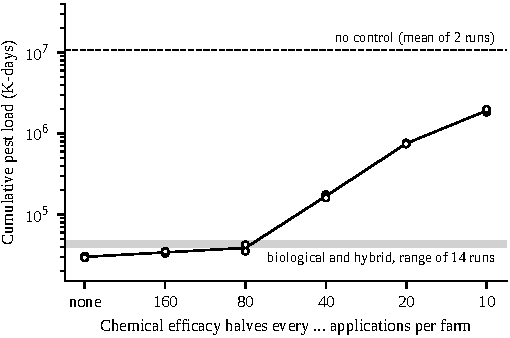
\includegraphics[width=0.7\textwidth]{figures/fig-decline}
		\caption{Chemical control on window A by efficacy-decline rate. Circles are single runs and the line joins means. The band is the range of 14 biological and hybrid runs at baseline. Fungal efficacy does not decline in these runs.}
		\label{fig:decline}
	\end{center}
\end{figure}

\subsection{The Hybrid Strategy}

The hybrid differs from biological control only where farms reach Level 3, and treating at Level 1 every 14 days kept them below it. In the sensitivity screen, the hybrid applied chemicals only where treatment was delayed: a trigger at Level 2 or 3, or re-treatment every 28 days. Rerun with non-declining chemical control, these settings gave a tie when treating only at Level 3 (ratios 0.89 to 1.04), and an ordering of chemical (262,998 K-days), hybrid (693,075), and biological (1,119,909) when re-treating every 28 days. While fungal efficacy holds, the hybrid adds nothing. It helps when both agents lose efficacy quickly.

\subsection{Sensitivity}

The baseline ranking, biological and hybrid tied, then chemical with decline 20, then no control, held in 15 of 18 cases (Table~\ref{table:oat}). No control was last in all 18. When treatment waited for Level 3 or was repeated every 28 days, biological control ranked first. When settlement survival was 0.01, chemical control ranked first, but the outbreak was about 26 times smaller, so this ranking is less certain. The response rules mattered more than any biological parameter: for biological control, waiting for Level 2 raised the load 16.6 times and waiting for Level 3, 33 times. Wind bias, long-jump rate, and the fungus-to-chemical ratio moved loads by less than 1.5 times. Runs with wind from the south-west gave 0.96 to 1.11 times the load of runs with wind from the north-east, inside the noise bands.

\begin{table}[!htbp]
\vspace{2ex}
\centering
\small
\caption{One-at-a-time screen on window A: largest change in load over the four strategies, as the absolute log$_{10}$ ratio to the baseline pool. One run per case. The ranking changed for settlement survival 0.01, a trigger at Level 3, and re-treatment every 28 days.}
\label{table:oat}
\begin{tabular}{lll}
\hline\hline
Assumption & Low, high & Change \\ \hline
Settlement survival & 0.01, 0.10 & 1.96 \\
Trigger level & 2, 3 & 1.81 \\
Re-treatment interval & 7, 28 d & 1.49 \\
Parasitism & 0, 0.668 & 1.16 \\
Neighbour transmission & $\times$0.25, $\times$4 & 0.86 \\
Level thresholds & $\times$0.5, $\times$2 & 0.59 \\
Long-jump probability & 0, 0.2 & 0.17 \\
Fungus-to-chemical ratio & 0.8, 1.0 & 0.17 \\
Wind bias & 0.5, 1.0 & 0.06 \\
\hline\hline
\end{tabular}
\end{table}

\subsection{Hindcast}

Table~\ref{table:hindcast} compares the model with the SRA record. At baseline the model spread too slowly: even without control it reached 0.30 of the validated area. A threefold transmission rate brought no control to 0.98 of it. That rate is one parameter tuned to one number with control ignored, and it was not used in the strategy comparison. The same run fell short earlier in the outbreak: 2,861 ha at the weekly output nearest 11 September 2025, against 4,923 ha recorded for Negros Island on that date \citep{MojicaSevilla2025}. No run matched which municipalities were worst affected (rank correlations of $-0.29$ to 0.22 outside the seeded units). In the hybrid run all infested farms stayed at Level 1, while the provincial survey found 53\%, 31\%, and 16\% of infested farmlots at Levels 1 to 3 \citep{PGNO2026}. Real response is slower and less complete than the model's weekly, error-free trigger: about 53\% of the validated area had been treated by 2 October 2026 \citep{SRA2026FOI}.

\begin{table}[!htbp]
\vspace{2ex}
\centering
\small
\caption{Hindcast, 2 October 2026: model cane area ever infested against the 72,103 ha validated by the SRA \citep{SRA2026FOI}. Hybrid: mean of two runs. Others: one run. $\rho$ is the Spearman correlation with the SRA share by municipality over the 45 unseeded units.}
\label{table:hindcast}
\begin{tabular}{lrrr}
\hline\hline
Run & Area (ha) & Ratio & $\rho$ \\ \hline
Hybrid, baseline & 2,908 & 0.04 & 0.10 \\
None, baseline & 21,275 & 0.30 & $-0.29$ \\
None, long jump 0.2 & 44,072 & 0.61 & 0.22 \\
None, transmission $\times$2.5 & 58,136 & 0.81 & $-0.09$ \\
None, transmission $\times$3 & 70,430 & 0.98 & $-0.18$ \\
None, transmission $\times$4 & 105,535 & 1.46 & $-0.04$ \\
\hline\hline
\end{tabular}
\end{table}

\subsection{Discussion}

Within its assumptions, the model suggests three things. Any control strategy reduces pest load far below no control. Acting early matters more than which agent is used: delaying the trigger or the re-treatment changed loads more than any biological parameter did. The ranking of chemical against biological control turns on two quantities that have not been measured, how fast chemical efficacy declines with repeated use and whether fungal efficacy holds. The biological lead holds only if fungal efficacy holds, and the hybrid is best only when both agents lose efficacy quickly.

The hindcast bounds how far these comparisons can be read. Baseline spread is too slow, the model does not reproduce which municipalities are worst affected, and its farmers respond more promptly than observed. The comparisons are therefore relative, between strategies run under the same assumptions. Data on the repeated-application efficacy of both agents, on spread between fields, and on the timing of real treatment would most change them.
 % DRAFT, 18 Nov 2026

		\makereferences{references}
	\end{mainmatter}
\end{document}
